We ran two types of tests to validate that preexisiting models worked and were
comparable to our proposed sensing matrices that combined the two types of
models. In one, we simulate compressed sensing by creating sensing operators,
measuring an image and then solving a TV-minimization problem to attempt to
recover the image. We then compare the recovered image to the original to
determine the relative error. Concretely, we compute the relative error
$\varepsilon$ as

\begin{equation}
  \frac{||x^{\#} - x||_2}{||x||_2} = \varepsilon
\end{equation}

and compare this error for each of the possible methods considered. In the other
test, we were only interested in the time to compute the solution $x^{\#}$ for
the various types of methods. In particular, we wanted to show that the
structured random matrices are much more efficient than using a completely
random matrix with Gaussian i.i.d. entries. In neither case is there any
appreciable amount of noise added to the measurements and in general we will
not show the reconstructed images since for our experiments the construction
quality was good enough across the board that differences between the images
were not meaningfully discernable. 

In the first experiment we tested our method on a $128 \times 128$ modified
Shepp-Logan phantom test image and used $128^2/3$ measurement samples for our
data to reconstruct the image. Figure \ref{fig:shepplogan} shows an example of
this image and its reconstruction.


\begin{figure}[h!]
  \centering
  \caption{Modified Shepp-Logan phantom reconstructed using a circulant matrix with RPMS restriction.}
  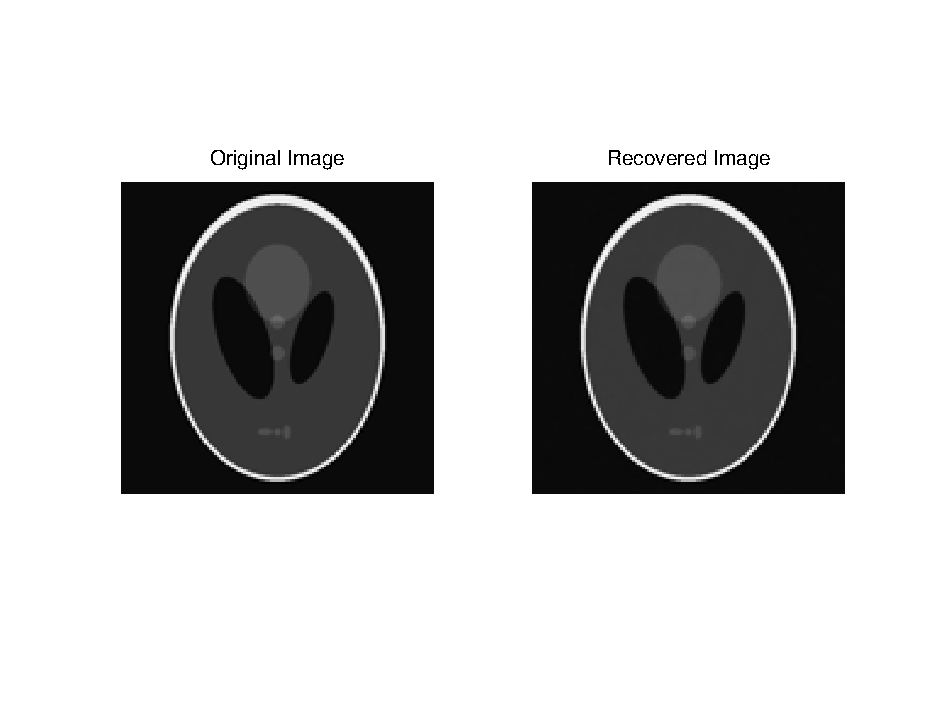
\includegraphics[width=0.6\textwidth, trim= 0 40 0 40, clip=true]{figs/rpms.pdf}
  \label{fig:shepplogan}
\end{figure}


\begin{table}[h] 
  \begin{tabular}{lll|lllll} 
    \textbf{Matrix Type}       & \textbf{Input Randomizer} & \textbf{Output Randomizer} & \textbf{Error} & \textbf{Time}  & \\ \hline
    \multirow{2}{*}{Circulant} & \multirow{2}{*}{N/A}      & Sub                        & 0.0156         & 4.97s          & \\
                               &                           & RPMS                       & 0.0159         & 7.80s          & \\ \hline
    \multirow{2}{*}{Toeplitz}  & \multirow{2}{*}{N/A}      & Sub                        & 0.0193         & 25.9s          & \\ 
                               &                           & RPMS                       & 0.0170         & 16.9s          & \\ \hline
    \multirow{4}{*}{Fourier}   & \multirow{2}{*}{Local}    & Sub                        & 0.0183         & 7.89s          & \\ 
                               &                           & RPMS                       & 0.0517         & 14.0s          & \\             
                               &  \multirow{2}{*}{Global}  & Sub                        & 0.0166         & 4.98s          & \\ 
                               &                           & RPMS                       & 0.0529         & 14.1s          & \\ \hline
    \multirow{4}{*}{Hadamard}  & \multirow{2}{*}{Local}    & Sub                        & 0.0167         & 552s           & \\
                               &                           & RPMS                       & 0.0153         & 752s           & \\
                               & \multirow{2}{*}{Global}   & Sub                        & 0.0157         & 544s           & \\
                               &                           & RPMS                       & 0.0137         & 782s           & \\
  \end{tabular} 
\caption{Table of reconstruction error $\varepsilon$ and timing results for all it the structured sensing matrices described previously.}
\label{tab:errors}
\end{table}

Table \ref{tab:errors} summarizes the results of our first experiment comparing
the solution accuracy of the various sensing matrices and input and output
randomizers. We do not use an input randomizer with circulant or Toeplitz
matrices since we could not converge to a solution using those methods. We see
that the reconstruction errors for almost all of the methods are comparable.
However, in the case of a Fourier transform sensing matrix with RPMS
subsampling operator does not work well. In addation to not achieving a
solution as good as the othertested methods, it showed poor convergence
compared to the simpler subsampling methods in the sense that it took longer to
converge. We are not convinced that the RPMS method is working in that case,
but that it is functioning correctly for circulant, Toeplitz and Hadamard
sensing matrices (where we are unaware of it having ever been used before). 

\begin{table}[h]
  \begin{tabular}{l|lllllll} 
    \textbf{Matrix Type} & Gaussian & Circulant & Toeplitz & Fourier & Hadamard \\ \hline
    \textbf{Time}        & 12.2s    & 1.65s     & 4.24s    & 1.50s   & 102s*    \\ 
  \end{tabular}
  \label{tab:times}
  \caption{ In this table we see how the time to compute the
    solution for a smaller problem using the random structured sensing
    operators compares with the time to compute the solution using a completely
    random matrix with Gaussian i.i.d. entries. *The fast Walsh-Hadamard
    transform in \textsc{Matlab} is written in \textsc{Matlab} and is slow.}
  \end{table}

In the second experiment we used the same test image scaled by a factor of a
half because the testing machine that we were using could not handle solving
the slightly larger (yet still small) problem using the completely random
matrix in  a reasonable amount of time. This was due to not only the complexity
of computing matrix-vector products with the random matrix, but also due to
memory restructions.

Table \ref{tab:times} summarizes the results of the second experiment. We see
that the the structured random matrices are able to compute the solution much
more quickly than the completely random matrix, with the exception of the
operator using the fast Walsh-Hadamard transform, which suffers from a slow
implementation in \textsc{Matlab}. However, the transform has the same
complexity as the FFT and so we expect that if the two were implemented
similarly, that thet should exhibit similar performance.  The Toeplitz based
sensing matrix is a little slower than the others using a fast transform, but
this is expected since performing a fast Toeplitz matrix-vector multiplication
requires using an FFT on a vector that is twice the size of the one you wish to
multiply. 

Overall the tests indicate the importance of the fast transforms for large
problems and the possibility of using the RPMS restriction operator with
sensing matrices other than circulant as originally suggested in
\cite{romberg2009}.
